\chapter{Autoencoders}

\section{Unservised Learning}
Mosto impressive results in deep learning have been obtained with \textbf{purely supervised learning} methods. In vision typically classification (e.g. object recognition).
Although progress has been slower, unsupervised learning is likely to remain important for future advances in deep learning. 

\begin{figure}[H]
    \centering
    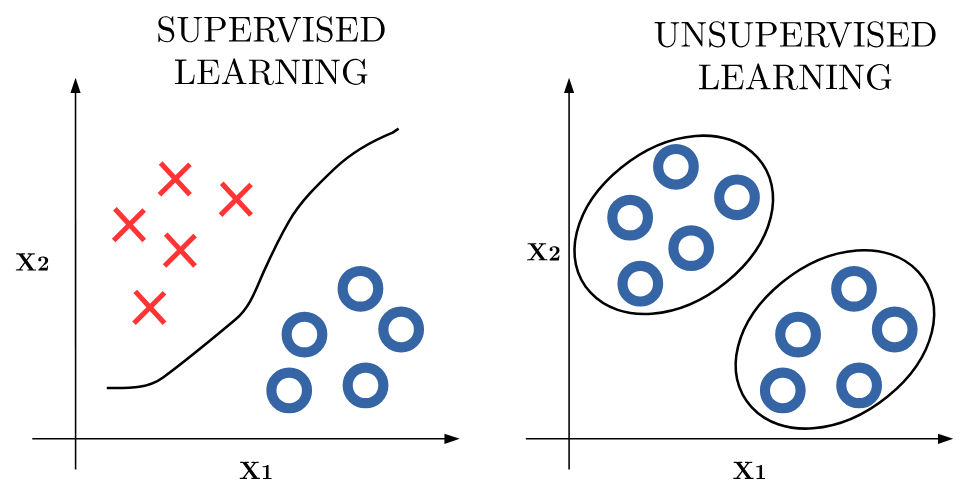
\includegraphics[width=0.5\textwidth]{images/supervised_unsupervised.png}
    \caption{Difference between supervised and unsupervised learning.}
    \label{fig:MHA2}
\end{figure}

\subsection{Why Unsupervised Learning?}
Deeper models lead to \textbf{more parameters}, which implies the requirement for \textbf{high number of training data} to avoid overfitting. The reason are:
\begin{enumerate}
    \item It is often easier to obtain unlabelled data then labeled data, which can require human annotation. We can also exploit unlabelled data, it is much more readibly and often free.
    \item Unsupervised learning involves observing several examples of a random vector $x$ and attempting to implicity or explicity learn the probability distribution $p(x)$, or some interesting properties of that distributions. We can capture enough information about the observed variables to ask new questions about them.
    \item Another two characteristic of unsupervised learning are:
        \begin{compactitemize}
            \item \textbf{Optimization}: unsupervised pre-training helps in initializing the parameters at a good position in the optimization landscape, significantly better than any position given by random inizialization.
            \item \textbf{Regularization}: unsupervised learning is a good regularizer for supervised learning, it helps in reducing overfitting. 
        \end{compactitemize}
\end{enumerate}
This advantage is evident in pratical applications, such as transfer learning and domain adaptation.
\begin{figure}[H]
    \centering
    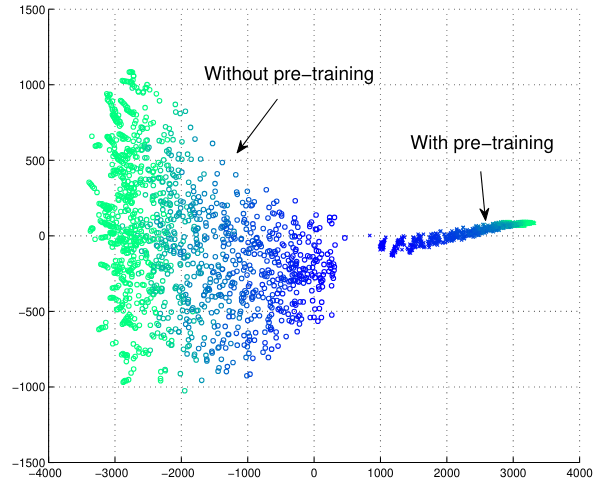
\includegraphics[width=0.35\textwidth]{images/SP.png}
    \caption{SOMAP embedding of functions represented by 50 networks w and w/o pre-training (Erhan et al., 2010).}
    \label{fig:MHA2}
\end{figure}

\section{Learning Rapresentations}
Take the \textbf{MNIST} dataset as an example, the image were centred in a $28x28$ image. Suppose each pixel is representable with a binary value: what is the cardinality of the whole set consisting of all the $28x28$ binary image?
\begin{equation}
    D^{i}_{2,784}=2^{28x28} = 2^{784}=1.01745...10^{236}
\end{equation}
The problem is that most of ${2}^{784}$, or more in general of $R^N$, consists of \textbf{invalid inputs}. 

Similary, if you generate a document by picking letters uniformly ar random, what is the probability that you will get a meaningful English-language text? \textbf{Almost zero}, because the distribution of natural leanguage sequences occupies a very little volume in total space of sequences of letters.
\newpage
\subsection{Manifold Assumption}
Many machine learning problems seem hopeless if we except the machine learning algorithm to learn functions with interesting variations across all of $R^N$.
\begin{wrapfigure}{r}{0.4\textwidth}
    \centering
    \vspace{-10pt}
    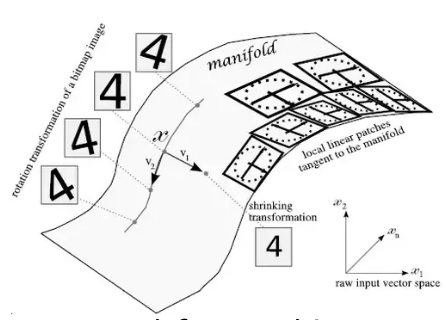
\includegraphics[width=\linewidth]{images/manifold.png}
    \label{fig:Scaled Dot Product Attention}
    \vspace{-10pt}
\end{wrapfigure}
\textbf{Manifold Assumption}: data lies approximately on a manifold of much lower dimension than the input space, where the actual degrees of freedom that can account for the variability in the data is \textbf{much lesser}.

When the data lies on a low-dimensional \textbf{manifold}, it can be most natural for machine learning algorithms to \textbf{REPRESENT} the data in terms of coordinates in the manifold than in terms of coordinates in $R^N$ .
\vspace{0.5cm}

To find a good representation of the data, it's better understand what we mean by \textbf{good representation}, so:
\begin{compactitemize}
    \item We are looking for a representation that \textbf{preserves as much information} about $x$ as possible while obeying some penalty or constraint.
    \item This additional constraint keep the learned representation \textbf{simple} or \textbf{more accessible} than $x$ itself.
    \item The new representation can be \textbf{task-specific} or \textbf{task-agnostic}.
\end{compactitemize}

\begin{infobox}[Difference between Task-specific and Task-agnostic]
    A \textbf{task-specific representation} is a representation of the data that is learned with the goal of performing well on a particular task, such as classification or segmentation. It keeps only the information that is directly useful for that task and may discard details that are irrelevant for it. Because of this, task-specific representations are usually very effective for the task they are designed for, but they do not generalize well to different tasks.

    A \textbf{task-agnostic representation}, instead, is learned without focusing on a particular task. Its goal is to capture general and meaningful structure in the data that can be reused for many different tasks. These representations are more flexible and transferable, but may be less optimal when applied to any single specific task compared to task-specific ones.
\end{infobox}

Beyond thus consideration, there are some \textbf{criteria} that a good representation should satisfy:
\begin{compactitemize}
    \item \textbf{Lower dimensional representation}: attempt to \textbf{compress} as much information as possible about $x$ in a smaller representation.
    \item \textbf{Sparse representation}: embed the dataset into a representation whose entries are \textbf{mostly zero} for most inputs.
    \item \textbf{Indipendent representation}: attempt to \textbf{disentangle} the factors of variatiom underlying the data distribution such that dimension of the representation are statistically independent.
\end{compactitemize}

\begin{infobox}[Sparse Representation Example]
    Consider an input image representing a handwritten digit. Instead of activating many features at once, a sparse representation will activate only a few neurons corresponding to specific local patterns (for example: one neuron for a vertical stroke, one for a curve, etc.). 
    
    \textbf{Example:}
    
    \[
    x = \text{image of "7"}
    \]
    Sparse code:
    \[
    z = [0, 0, 1.2, 0, 0, 0.8, 0, 0, 0, 0]
    \]
    
    Only the features for \textit{"vertical line"} and \textit{"diagonal stroke"} are active. All others remain zero (or close to zero).
\end{infobox}

\begin{infobox}[Independent (Disentangled) Representation Example]
    Here, each dimension of the representation corresponds to a different \textbf{independent factor of variation} in the data.
    
    \textbf{Example:} Consider faces. A disentangled representation might separate:
    \begin{compactitemize}
        \item Identity
        \item Expression (smiling vs. neutral)
        \item Lighting direction
    \end{compactitemize}
    
    So a representation could look like:
    
    \[
    z = [\text{identity}, \text{smile intensity}, \text{light angle}]
    \]
    
    Changing one value (e.g., smile intensity) does \textbf{not} affect the others. Each factor is represented independently.
\end{infobox}
    
\subsection{Dimensionality Reduction}
\textbf{Dimensionality Reduction techniques} often create low-dimensional representations in which elements have \textbf{fewer or weaker dependencies} than the original high-dimensional data. When a model is forced to compress input data, it implicitly identifies and removes \textbf{redundancies} while discarding the least amount of information possible. In this context, \textbf{Principal Component Analysis (PCA)} can be viewed as an unsupervised learning algorithm that learns a low-dimensional representation of data whose elements have \textbf{no linear correlation} with each other.

\begin{wrapfigure}{r}{0.4\textwidth}
    \centering
    \vspace{-10pt}
    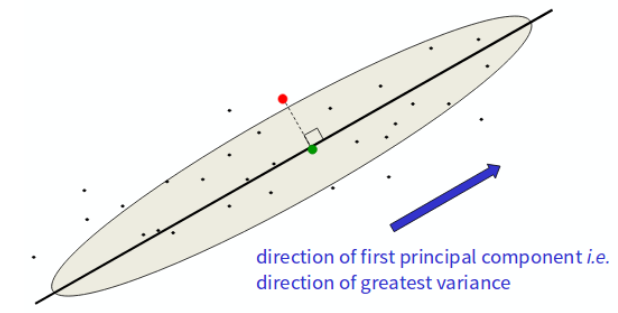
\includegraphics[width=\linewidth]{images/PCA.png}
    \label{fig:Scaled Dot Product Attention}
    \vspace{-10pt}
\end{wrapfigure}
PCA learns an \textbf{orthogonal, linear transformation} of the data that projects an input $\mathbf{x}$ to a \textbf{low-dimensional representation $\mathbf{z}$}, which lies in the subspace spanned by the \textbf{principal components}.
PCA works well \textbf{only} if the data is near a \textbf{linear manifold} in high-dimensional space.
We are interested in learning representations that \textbf{disentangle} more \textbf{complicated forms of feature dependencies}.
For this purpose, we need more than what can be done with a \textbf{simple linear transformation}.

\subsection{An inefficient way to fit PCA}
\begin{wrapfigure}{r}{0.4\textwidth}
    \centering
    \vspace{-10pt}
    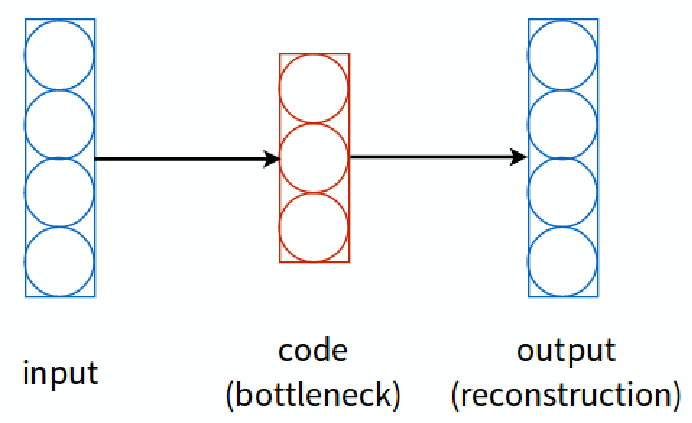
\includegraphics[width=\linewidth]{images/Bottleneck_layer.png}
    \label{fig:An inefficient way to fit PCA}
    \vspace{-10pt}
\end{wrapfigure}
The idea is to train a neural network with a \textbf{"bottleneck" hidden layer} having $M$ units and try to make the output ($\hat{\mathbf{x}}$) the same as the input ($\mathbf{x}$).
If the hidden and output layers are \textbf{linear}, and we minimize the squared reconstruction error:
\[
\min \left\| \hat{\mathbf{x}} - \mathbf{x} \right\|^2
\]
The $M$ hidden units will span the \textbf{same subspace} as the first $M$ principal components.
However:
\begin{compactitemize}
    \item Their \textbf{weight vectors} will \textbf{not be orthogonal}.
    \item They will have approximately \textbf{equal variance}.
\end{compactitemize}

\section{Autoencoders}
\begin{wrapfigure}{r}{0.4\textwidth}
    \centering
    \vspace{-10pt}
    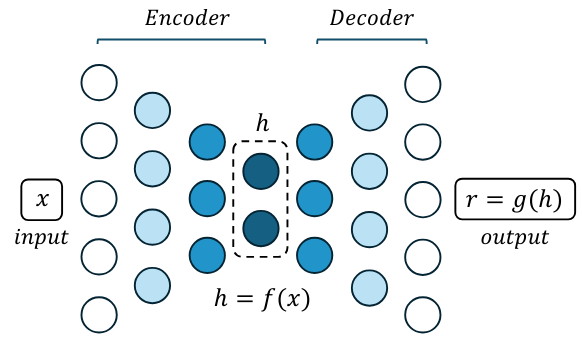
\includegraphics[width=\linewidth]{images/autoencoder+.png}
    \label{fig:Scaled Dot Product Attention}
    \vspace{-10pt}
\end{wrapfigure}
An \textbf{autoencoder} is a feed-forward neural network trained to attempt to copy its input to its output.
The network may be viewed as a consisting of two parts: an \textbf{encoder} function $h=f(x)$ and a \textbf{decoder} that produces a reconstruction $r=g(h)$.
The aim is to induce in $h$ useful properties and the most salient features of the training data.

\begin{figure}[H]
    \centering
    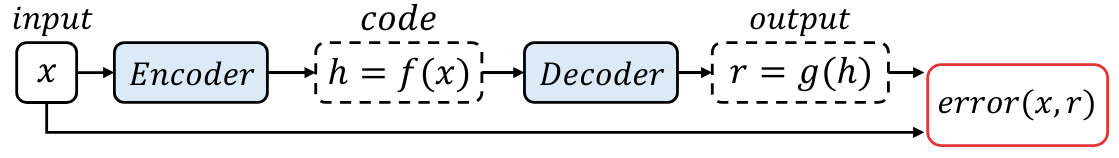
\includegraphics[width=0.6\textwidth]{images/autoendoer_pipeline.png}
    \caption{Autoencoders Pipeline}
    \label{fig:MHA2}
\end{figure}
\newpage
With \textbf{nonlinear layers} before and after the code , it should be possible to represent data on or near a \textbf{nonlinear manifold}. The \textbf{encoder} maps from the data space ($\mathbf{x}$) to the \textbf{coordinates on the manifold} ($\mathbf{z}$). The \textbf{decoder} performs the \textbf{inverse transformation} ($\hat{\mathbf{x}}$). Both the encoder and the decoder can be rich, \textbf{multi-layer functions}.

\subsection{Risk: Learning the Identity Function}
\begin{wrapfigure}{r}{0.25\textwidth}
    \centering
    \vspace{-10pt}
    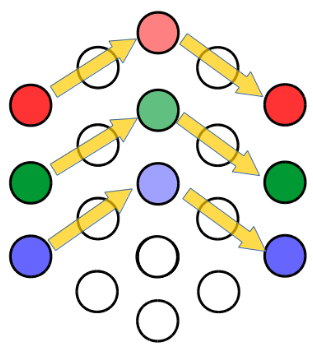
\includegraphics[width=\linewidth]{images/identity.png}
    \label{fig:Scaled Dot Product Attention}
    \vspace{-10pt}
\end{wrapfigure}
What we mean by \textbf{overfitting} in autoencoders is slightly different from classic Neural Networks (NNs). Here, the risk is not merely memorizing every single data point, but rather learning a trivial function that maps $g(f(\mathbf{x}))=\mathbf{x}$ everywhere.
Therefore, the model does not effectively \textbf{compress} the data; it simply \textbf{copies} the input to the output.
This eventually can occur if the encoder and decoder are given \textbf{too much capacity} (e.g., if the hidden layers are too large or deep), or if the hidden code has a dimension \textbf{greater than the input} (an overcomplete code), which facilitates the learning of the identity function.

\subsection{Undercomplete Autoencoders}
The first attempt at autoencoder regularization is to constrain $h$ to have a \textbf{smaller} dimension than $x$.
Learning an \textbf{undercomplete} representation forces the autoencoder to capture the most salient factors of data variation.
The learning process plans to minimize:
\begin{equation}
    L(x,g(f(x)))
\end{equation}
where $L$ is a loss function penalizing $g(f(x))$ for being dissimilar from $x$ (e.g. MSE).

\textbf{Problem}: if the encoder and decoder are allowed too much capacity, an undercomplete autoencoder can learn to perform the copying task without extracting useful information.
\begin{figure}[H]
    \centering
    \begin{minipage}{0.45\textwidth}
        \centering
        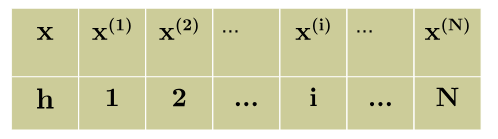
\includegraphics[width=\textwidth]{images/UA2.png}
        \label{fig:Trend_Seasonality}
    \end{minipage}
    \hfill
    \begin{minipage}{0.45\textwidth}
        \centering
        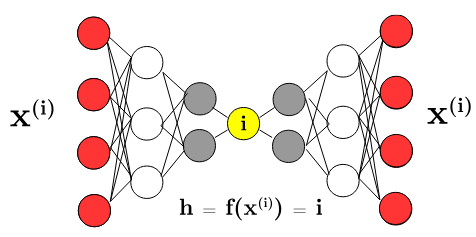
\includegraphics[width=\textwidth]{images/UA.png}
        \label{fig:Residuals}
    \end{minipage}
    \label{fig:TS_Residuals}
\end{figure}

\section{Regularized Autoencoders}
The fundamental tension in autoencoder design parallels general machine learning: insufficient capacity causes underfitting, while excessive capacity enables learning the identity function. Deep learning principles suggest using large models with sufficient capacity to fit complex functions, but constraining them through regularization to use this power wisely. 
Regularized autoencoders use a loss function that encourages the model to have other properties besides tha ability to copy its input to its output.
Beacause the model is \textbf{forces to prioritize} which aspects of the input should be copied, it often learns \textbf{useful properties} of the data.
It can capture the structure of the data-generating distribution due to \textbf{opposition} between reconstruction distribution and regularizer.


\subsection{Sparse Autoencoders} 
\begin{wrapfigure}{r}{0.25\textwidth}
    \centering
    \vspace{-10pt}
    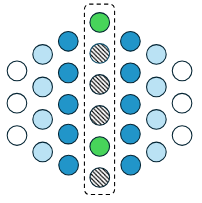
\includegraphics[width=\linewidth]{images/SA.png}
    \label{fig:Scaled Dot Product Attention}
    \vspace{-10pt}
\end{wrapfigure}
A \textbf{sparse autoencoder} is an autoencoder whose training criteretion involves an additional \textbf{sparsity penalty} on the code layer $h$. 
\begin{equation} L_{SAE} = D(x, g(f(x))) + \lambda \|h\|_{1} \end{equation} 
Thanks to the sparsity penalty, we can build an over-complete representation of the input data without the risk of learning the identity function. Sparse autoencoders are typically used to learn features for another rask, such as \textbf{classification}.


\begin{infobox}[Where the regularization is applied?]
    In a sparse autoencoder, the regularization is applied \textbf{directly on the activations of the code layer $h$}, not on the weights. This differs from typical weight regularization (like $L_1$ or $L_2$ penalties on $W$), which constrains the magnitude of the parameters. 
    
    By penalizing the activations instead, the model is forced to activate only a few neurons for each input, learning a \textbf{sparse representation} even if the network has many hidden units.
\end{infobox}
    
\begin{infobox}[The size of code layer]
    The code layer $h$ in a sparse autoencoder is often \textbf{larger than the input layer}, creating an \textbf{over-complete representation}. 
    
    Even though there are more neurons than input dimensions, the sparsity penalty ensures that for each input, only a small subset of neurons is active. This allows the autoencoder to learn richer, more disentangled features without simply copying the input.
\end{infobox}
\begin{wrapfigure}{r}{0.35\textwidth}
    \centering
    \vspace{-10pt}
    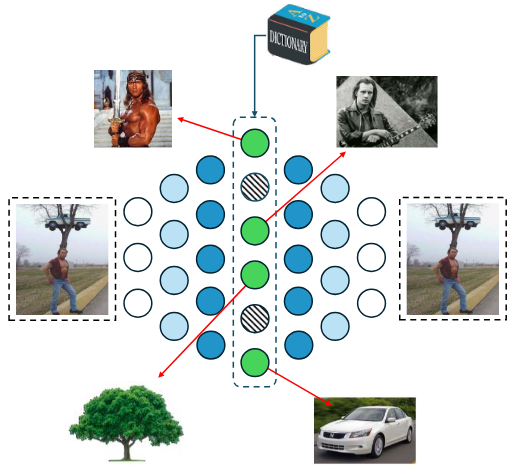
\includegraphics[width=\linewidth]{images/SA_idea.png}
    \label{fig:Scaled Dot Product Attention}
    \vspace{-10pt}
\end{wrapfigure}
Sparse autoencoders can discover representa-tions that account for most or all information on a signal with a combination of a small num-ber of elementary, recurrent, and only partially related concepts.
Given the input signal, the general idea is to find a short list of terms that best describes the input from a \textbf{learned dictionary}.
The new representation h has the dimensionality of the dictionary, much higher than the dimen- sionality of the input (overcompleteness)

\subsection{Denoising Autoencoders}
\begin{wrapfigure}{r}{0.4\textwidth}
    \centering
    \vspace{-10pt}
    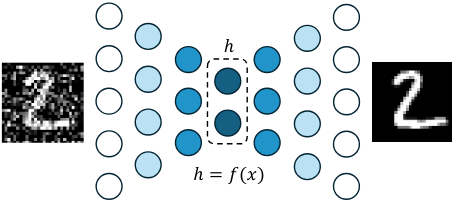
\includegraphics[width=\linewidth]{images/DA.png}
    \label{fig:Scaled Dot Product Attention}
    \vspace{-10pt}
\end{wrapfigure}
To force to discover more \textbf{robust features}, a \textbf{denoising autoencoder} reconstruct the input $x$ from a  \textbf{corrupted version} $\hat{x}$ of it.
\begin{equation}
    L_{DAE}=D(x,g(f(\hat{x}))) e.g., \hat{x} \sim N(x,\sigma^2 I)
\end{equation}
The corrupted input $\hat{x}$ can be obtained by applying on $x$ some form of noise, for example, additive white gaussian noise or dropout.

Denoising autoencoders must therefore \textbf{undo} this corruption rather than simply copying their input.

\begin{infobox}[The size of code layer]
    In Denoising Autoencoders, unlike Sparse Autoencoders, the number of neurons in the code layer is usually smaller than the input layer. 
    This is because each neuron in the code layer is activated by the input, and having a code larger than the input could lead the model to simply learn the identity function.
\end{infobox}

\begin{wrapfigure}{r}{0.5\textwidth}
    \centering
    \vspace{-10pt}
    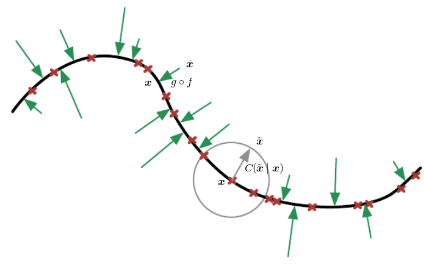
\includegraphics[width=\linewidth]{images/FV.png}
    \label{fig:Scaled Dot Product Attention}
    \vspace{-10pt}
\end{wrapfigure}
A \textbf{Denoising Autoencoder (DAE)} is able to bring $\hat{x}$ back to the ``curve'' point 
where the original $x$ resides. In other words, it \textbf{learns a vector field towards higher probability regions}. 

By knowing, for each point near the curve, where it should be projected, a DAE has \textbf{implicitly learned the structure of the underlying manifold} responsible for the data-generating process. 

The \textbf{denoising training} forces the encoder and decoder to \textbf{implicitly capture the structure of the probability distribution} $p_{\text{data}}(x)$.

\subsubsection{Denoising Autoencoders for Anomaly Detection}
\textbf{Denoising Autoencoders (DAE)} learn to reconstruct samples that lie on the \textbf{data manifold} by removing noise from the input.

\textbf{Key insight:} During training, the model learns the \textbf{typical structure of normal data}. 
When presented with an \textbf{anomalous sample}, its reconstruction error becomes significantly higher, because the anomaly does not lie on the learned manifold.

\textbf{DAEs for Anomaly Detection: how they work:}
\begin{compactitemize}
    \item Train the DAE with \textbf{noisy versions of normal data}.
    \item At inference, compute the \textbf{reconstruction error} $e(x) = \|x - \hat{x}\|_2$.
    \item Flag samples with \textbf{high $e(x)$} as potential anomalies.
\end{compactitemize}

\subsection{Contractive Autoencoders}
A \textbf{contractive autoencoder} is an autoencoder that reconstructs the input from the code and makes the \textbf{code insensitive} to the input.
\begin{equation}
    L_{CAE} = D(x, g(f(x))) + \lambda \left\| \frac{\partial f(x)}{\partial x} \right\|_2
\end{equation}
The regularization term encourages the gradient of the hidden layer with respect to inputs to be small. This forces the model to:
\begin{compactitemize}
    \item learn a function that \textbf{does not change much} when $x$ changes slightly or is affected by small perturbations.
    \item reduces the number of effective degrees of freedom of the representation.
    \item represent only the variations that are needed to reconstruct training examples.
\end{compactitemize}

\vspace{0.2cm}
\begin{wrapfigure}{r}{0.4\textwidth}
    \centering
    \vspace{-10pt}
    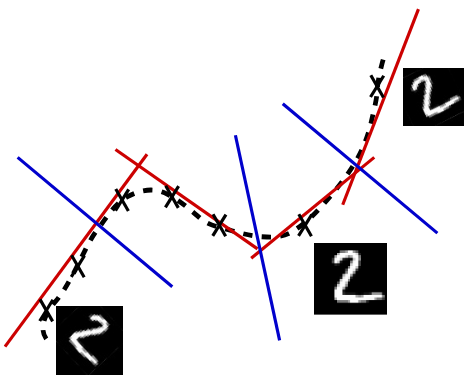
\includegraphics[width=\linewidth]{images/CA.png}
    \label{fig:Scaled Dot Product Attention}
    \vspace{-10pt}
\end{wrapfigure}
We wish to extract features that only reflect variations observed in the training set.

With the \textcolor{red}{red line}, we indicate directions of variations for which the encoder needs to be sensitive to reconstruct well input.

With the \textcolor{blue}{blue line} line, we indicate directions of variations for which the encoder doesn’t need to be sensitive because they are not observed in the training set.

The name \textbf{Contractive Autoencoder (CAE)} arises from the way that the CAE \textbf{warps space}. 
Because the CAE is trained to \textbf{resist perturbations of its input}, it is encouraged to map a neighborhood of input points to a \textbf{smaller neighborhood of output points}. 
Thanks to the \textbf{contractive term}, the model becomes \textbf{invariant to small perturbations} near the points.

As is the case for \textbf{Denoising Autoencoders}, a CAE knows the \textbf{tangent planes} at each location of the underlying manifold. 
In this way, it can \textbf{capture the manifold structure of the data}.
